%% This LaTeX-file was created by <wiera> Mon Oct  9 18:45:08 2000
%% LyX 0.12 (C) 1995-1998 by Matthias Ettrich and the LyX Team

%% Do not edit this file unless you know what you are doing.
\documentclass[a4paper,english]{report}
\usepackage[T1]{fontenc}
\usepackage[latin1]{inputenc}
\usepackage{babel}
\usepackage{graphics}

\makeatletter


%%%%%%%%%%%%%%%%%%%%%%%%%%%%%% LyX specific LaTeX commands.
\newcommand{\LyX}{L\kern-.1667em\lower.25em\hbox{Y}\kern-.125emX\spacefactor1000}

%%%%%%%%%%%%%%%%%%%%%%%%%%%%%% Textclass specific LaTeX commands.
\newenvironment{lyxcode}
  {\begin{list}{}{
    \setlength{\rightmargin}{\leftmargin}
    \raggedright
    \setlength{\itemsep}{0pt}
    \setlength{\parsep}{0pt}
    \ttfamily}%
   \item[]}
  {\end{list}}

%%%%%%%%%%%%%%%%%%%%%%%%%%%%%% User specified LaTeX commands.
\usepackage{textcomp}
\makeatother

\begin{document}


\title{Diploma Thesis:\\
Utility Support for Checking OCL Business Rules in Java Programs}


\author{Ralf Wiebicke}


\date{May 2000}

\maketitle

\section*{Copyright}

Copyright \copyright~2000 Ralf Wiebicke.

Permission is granted to copy, distribute and/or modify this document under
the terms of the GNU Free Documentation License, Version 1.1 or any later version
published by the Free Software Foundation; with no Invariant Sections, no Front-Cover
Texts, and no Back-Cover Texts. A copy of the license is available at http://www.gnu.org/copyleft/fdl.html.

The source code developed together with this paper is Copyright \copyright~2000
Ralf Wiebicke and published under the GNU Lesser General Public License (LGPL).
Additional source code was developed by Steffen Zschaler under LGPL.


\section*{Availability}

This document is available at http://dresden-ocl.sourceforge.net/diploma\_rw7/
in several electronic forms including \LaTeX{}, Postscript, PDF, Html and the
original kLyx version. 

The source code developed together with this paper is available at http://dresden-ocl.sourceforge.net/.


\section*{Neu}

\begin{enumerate}
\item Section \ref{Sec:WrapperLoop}. Avoiding the Wrapper Loop
\item Chapter 2 ``Related Work''
\item Sections \ref{sec: ReverseEngineeringWomble} and following.
\item Section \ref{sec: compareJass}.
\end{enumerate}
\tableofcontents


\chapter{Introduction}

Wishlist in \cite{ff3} section 3.6.


\chapter{Related Work}


\section{Constraint Checkers}

JMSAssert (\cite{JMSAssert}) provides OCL for java. Constraints are embedded
into java doc comments. The tool links into the JVM to make the constraints
checked. This approach does not involve source code modification. This makes
it easier to use, but also platform dependent (currently Windows only). It also
requires just-in-time compilers to be switched off. Binaries are available at
no cost.

Also Cybernetic Intelligence develops an OCL compiler (\cite{Cybernetic}).
The current prototype claims to support syntax checking only. Type checking
is under development. Frontends are available for Select Enterprise and Rational
Rose.

Elixir claims OCL support in it's CASE tool and it's java IDE. The CASE tool
provides an ocl text field only, without any syntax checking. For the IDE a
plugin is provided to integrate iContract (\cite{iContract}).

For some applications OCL is just too powerful. A simpler approach is demonstrated
in \cite{kbeans}. It implements a number of predefined constraint types, such
as \emph{numeric range} or \emph{ordering of arrays}. For instance to have an
attribute \texttt{age} constrained to positive values, one just adds a method
\texttt{getAgeMinValue()~\{return~0;\}}. Most OCL constraints I used in the
development of the ocl toolkit also could have been expressed with such simple
means. Constrained classes must be valid JavaBeans. Also, the class must announce
the change of attributes manually. KBeans is released under GPL. Additionally
there is a GUI for simulating an object population and checking constraints
against it.


\section{Code Instrumentation}

Jass (\cite{jassWeb}) is a preprocessor for java assertions developed at the
University of Oldenburg (\cite{jassDiplom}). Apart from class invariants and
method pre/postconditions it provides check statements (like assert() in C++)
and loop invariants/variants. Assertions are expressed in java, extended by
universal and existential quantifiers. Jass approaches a task similarly to code
injection presented in this paper with different means. Section \ref{sec: compareJass}
provides a detailed comparison. Jass is available under GPL.

There is a universal code instrumentation toolkit (\cite{CodeInstrumentation})
for java available. It parses java files into parse trees, preserving white
space and comments. The parse tree can be modified and written back into the
file. There are various applications for this, including tracing of program
execution. The code injection presented in this paper could probably realized
using this tool. However, the parser reads the full java structure, thus is
much more heavy-weight than the parser developed with this paper. There is a
test version available at no cost, limited in the size of source programs it
can handle.


\section{Reverse Engineering}

A powerful approach to reverse engineering has been developed at the MIT \cite{womble}.
The tool superwomble extracts an object model from java byte code. Object models
are roughly a subset of UML class diagrams, featuring inheritance and object
associations. An important challenge for the analysis is the detection of element
types of container attributes. The tool performs this very efficiently, without
requiring any additional help from the user. Thus, it complements the two approaches
presented in this paper. A detailed comparison is provided in section \ref{Sec:ReverseEngineering}.

JVision \cite{jvision} produces class diagrams from java source or byte code.
It's easy to use and has nice auto-layout. But it does not handle associations
in any way. Collection attributes are simply shown as attributes. Instead it
analyses, which classes create/use each other. This is not nearly as useful
as associations.


\chapter{Code Injection}

Injection of generated code into java programs is the main subject of this paper.
It covers anything beyond code generation, to get a java model checking its
own constraints. For an idea, where code generation ends and injection starts,
see section \ref{Sec:codegeneration_result}. 

This is followed by an analysis of requirements for the code injection and resulting
design decisions in section \ref{Sec:injection_requirements}. Section \ref{Sec:wrappingMethods}
describes the solution in detail. Section \ref{sec: compareJass} compares this
solution to Jass (\cite{jassWeb}) which approaches a similar task quite differently.

Finally sections \ref{Sec:temporalScope} and \ref{Sec:structuralScope} discuss
the more fundamental issue, when and how often invariants have to be checked.


\section{Results of Code Generation\label{Sec:codegeneration_result}}

The java code generator developed in \cite{ff3} produces a set of code fragments\footnote{
see class \texttt{tudresden.ocl.codegen.CodeFragment.}
}. These code fragment have the following properties:

\vspace{0.3cm}
{\centering \begin{tabular}{|l|p{70mm}|}
\hline 
Property &
\\
\hline 
\hline 
Constrained~type &
The default navigation context of this constraint.\\
\hline 
Kind &
Specifies, whether this constraint is an invariant, a pre- or a postcondition.
\\
\hline 
Constrained~operation &
The operation, this constraint applies to (valid for pre- and postconditions
only).\\
\hline 
Code &
Contains the actual java code to be executed.\\
\hline 
Result~variable &
Specifies the boolean value, which contains the result of the ocl expression
after code execution.\\
\hline 
\end{tabular}\par}
\vspace{0.3cm}

For each postcondition containing a @pre expression there are two additional
codefragments called preparation and transfer. See below.


\subsection{Preparation and Transfer Fragments}

The meaning of preparation and transfer fragments is explained on a dramatically
simplified example. 

Suppose a post condition for operation \texttt{employ()}, that leaves the attribute
\texttt{age} unchanged:

\begin{lyxcode}
context~Person::employ()~\\
post:~age=age@pre
\end{lyxcode}
the following codefragments will be produced:

\vspace{0.3cm}
{\centering \begin{tabular}{ll}
\hline 
Kind&
 Code\\
\hline 
\hline 
Transfer&
\texttt{int~node1;} \\
\hline 
Preparation&
\texttt{node1=this.age;}\\
\hline 
Post Condition&
\texttt{int~node2=this.age;}\\
&
\texttt{boolean~result=(node1==node2)}\\
\hline 
\end{tabular}\par}
\vspace{0.3cm}

Typically these fragments would be injected as follows:

\begin{lyxcode}
class~Person\\
\{\\
~~void~employ()\\
~~\{\\
~~~~int~node1;~~~~~~~//~transfer~fragment\\
~~~~node1=this.age;~~//~preparation~fragment\\
~~~~//~original~code~of~employ()\\
~~~~//~post~condition~fragment\\
~~~~node2=this.age;\\
~~~~boolean~result=(node1==node2)\\
~~\}\\
\}
\end{lyxcode}
Note, that precise semantics of codefragments involving the @pre expression
has been changed, so that the original meaning described in \cite{ff3} section
7.1.2 is no longer fully correct. For a detailed comparison see section \ref{Sec:maintainJavaCodeGenerator}.

\begin{lyxcode}
~
\end{lyxcode}

\section{Requirements and Design Decisions\label{Sec:injection_requirements}}

This section analyzes the requirements for the injector tool and derives some
fundamental design decisions.


\subsection{Reversable Modification\label{Sec:injection_requirements_reversable}}

The most important feature is the reversability of code injection. It must be
possible to

\begin{itemize}
\item Clean the code tracelessly from all injected fragments.
\item Redo the injection on source code that has already been modified, for instance
when constraints have been changed. 
\item Edit the modified source code without losing all changes at the next injection. 
\end{itemize}
These requirements makes things quite a bit more difficult, but there are serious
reasons for this. Otherwise there would be two versions of source code: the
original and the modified version. This raises some unpleasant problems:

\begin{enumerate}
\item Configuration management must handle two source code trees.
\item Developers must be careful to edit the original version only.
\item Running the ocl injector is required after every change of the java source code,
not only when the constraints have been changed. 
\item Stack traces of runtime exceptions point to the modified source code. Developers
must look for the corresponding place in the original version.
\end{enumerate}
The implementation of reversable modification requires a strategy of minimally
invasive modification. This is realized by two design decisions:

\begin{enumerate}
\item Method wrappers, explained detailed in section \ref{Sec:wrappingMethods}.
\item Explicit package qualifiers for the ocl library in the generated code. Otherwise,
an import statement for the ocl library would be necessary. This would be just
another spot, were the original source code had to be touched. Additionally,
this may introduce name conflicts beetween ocl library and user code.
\end{enumerate}

\subsection{Embedding Constraints in Java Source Code.\label{Sec:embedConstraints}}

It should be possible to embed constraints in the java documentation comments.
The placement of embedded constraints implicates (and replaces) the context
of the constraint. See the example below.

\begin{lyxcode}
/{*}{*}\\
~~~@invariant~ageGreaterZero:~age>0\\
{*}/\\
class~Person\\
\{\\
~~int~age;\\
~\\
~~/{*}{*}\\
~~~~~@postcondition:~age=age@pre\\
~~{*}/\\
~~void~employ();\\
\}
\end{lyxcode}
It is necessary to put the constraints directly under the nose of the developer.
The author is strongly convinced, that constraints stored in an extra text file
are too far away from attention.

Invariants may also placed on an attribute or method of their context class.
This is for convenience, since most invariants are clearly related to one specific
attribute or method.


\subsection{Checking the Element Type.}

The injected code must check, that collection attributes comply to the \texttt{@element-type}
and \texttt{@key-type} tags introduced in section \ref{Sec:element_type_tag}.
This is quite easily done just before checking invariants.

Note, that this feature may be be used standalone, without ocl expressions at
all. Then it provides a runtime check for typed collections.


\section{Code Insertion\label{Sec:wrappingMethods}}

The main task of code injection is to have some code executed immediately before
and after all methods (and after all constructors too). This section describes,
how this is done by the ocl injector.


\subsection{A Simple Approach\label{sec: SimpleApproach}}

A straight-forward solution would add the code directly into the method. But
this raises some severe problems. 

\begin{enumerate}
\item The code to be executed after the method (postcondition and invariants) has
to be inserted before any return statement.
\item The post condition code must have the return value available. Thus, a return
expression has to be computed in advance, if the post condition code refers
to the return value and/or the the return expression produces side effects.
\item There may be name conflicts beetween the original and the generated code, since
the generated code defines local variables.
\item For methods with return type void it must be decided, whether the post condition
code has to be inserted at the end of the method. This depends on whether the
end of the method is a reachable point of code. For the decision it needs a
complete control flow analysis of the method. Note, that if the post condition
code is wrongly inserted at the end of the method, the java compiler will fail
due to unreachable statements.
\end{enumerate}
An implementation would need a complete java parser, which touches the original
code at many different places and in a complicated way. This runs contrary to
the strategy of minimally invasive modification as decided in section \ref{Sec:injection_requirements_reversable}. 

Additionally, item 4 requires much of the semantic analysis performed by a java
compiler. This makes the simple approach very hard to implement. 

Jass (\cite{jassWeb}) uses this simple approach, and encounters all the problems
mentioned above. For a detailed comparison see section \ref{sec: compareJass}.

Method wrappers solve all these problems in a nifty but simple way.


\subsection{Wrapping Methods\label{Sec:wrappingMethodsSub}}

Some code tells more than thousand words, so I use an example to explain. Consider
the following method.

\begin{lyxcode}
int~someMethod(double~x)\\
\{\\
~~//~here~comes~the~code.\\
\}~
\end{lyxcode}
The code injector transforms this into two methods.

\begin{lyxcode}
int~someMethod\_wrappedbyocl\footnote{
This is not yet the full truth, see section \ref{Sec:WrapperLoop}.
}(double~x)\\
\{\\
~~//~here~comes~the~code.\\
\}\\
~\\
int~someMethod(double~x)\\
\{\\
~~//~some~code~checking~invariants/preconditions.\\
~~int~result=someMethod\_wrappedbyocl(x);\\
~~//~some~code~checking~invariants/postconditions.\\
~~return~result;\\
\}
\end{lyxcode}
Now let's have a look back at the problems encountered for the simple approach.
Non of them exists anymore. 

\begin{itemize}
\item The code to be executed after the method has to be inserted once only.
\item When the post condition code is executed, the return expression is already evaluated
and ready to use.
\item No name conflicts are possible, since user code and generated code are strictly
separated into different methods.
\item No control flow analysis is needed.
\end{itemize}
The user code is modified in a simple way: a suffix is appended to the method
name. For an implementation a very inchoate java parser is sufficient, which
understands ``java meta level'' only. The meta level covers anything outside
of method bodies and attribute initializers. This is a very small part of the
java language and easily to be analyzed by a hand-crafted parser. See section
\ref{sec: JavaParser} how easy it is.

This kind of method wrapping still has a problem, I called the wrapper loop.
See section \ref{Sec:WrapperLoop} how this is solved.


\subsection{Wrapping Constructors}

Another transformation is used for constructors, since they cannot be renamed.
Suppose a example constructor

\begin{lyxcode}
SomeClass(String~x)\\
\{\\
~~//~here~comes~the~code\\
\}
\end{lyxcode}
Instead of renaming, the original constructor gets an additional dummy argument.

\begin{lyxcode}
SomeClass(String~x,~Dummy\footnote{
Actually this is class \texttt{tudresden.ocl.injection.lib.WrapperDummy}.
}~oclwrapperdummy)\\
\{\\
~~//~here~comes~the~code\\
\}\\
~\\
SomeClass(String~x)\\
\{\\
~~this(x,~(Dummy)null);\\
~~//~some~code~checking~invariants.\\
\}
\end{lyxcode}
A special case occurs if a class provides no explicit constructor. Then there
is the default constructor as specified in \cite{JAVA} section 8.6.7. This
default constructor is not wrapped, but replaced by an explicit constructor
with the same access modifier.


\subsection{Avoiding the Wrapper Loop\label{Sec:WrapperLoop}}

Wrapping methods as described in section \ref{Sec:wrappingMethodsSub} causes
a problem for a special situation. This sections describes this situation and
the solution provided by the ocl injector.

The critical situation is shown in the figure below:

\vspace{0.3cm}
{\centering \resizebox*{!}{5cm}{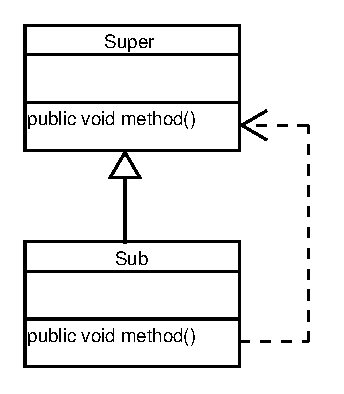
\includegraphics{WrapperLoop1.eps}} \par}
\vspace{0.3cm}

The dotted arrow represents a method call: \texttt{Sub.method()} contains a
statement \texttt{super.method();} somewhere.

The ocl injector changes the structure as shown below:

\vspace{0.3cm}
{\centering \resizebox*{!}{5cm}{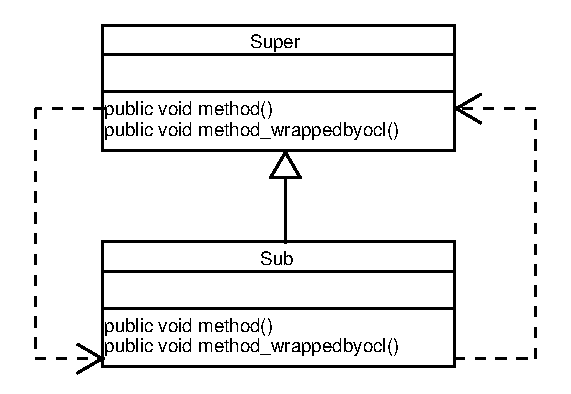
\includegraphics{WrapperLoop2.eps}} \par}
\vspace{0.3cm}

The arrows show the problem: there's an infinite loop of method calls. In detail
the following happens:

\begin{enumerate}
\item Method \texttt{Sub.method()} is called somewhere in the user program. This is
a wrapper method replacing the original method, which is named \texttt{method\_wrappedbyocl()}
now.
\item \texttt{Sub.method()} does some ocl specific things, before it executes the
statement \texttt{method\_wrappedbyocl()}. This calls the original method \texttt{Sub.method\_wrappedbyocl()}
as it is supposed to be.
\item \texttt{Sub.method\_wrappedbyocl()} contains the \texttt{super.method();} statement,
therefore calls \texttt{Super.method()}.
\item \texttt{Super.method()} is a wrapper method replacing the original method, which
is called \texttt{Super.method\_wrappedbyocl()} now. It does some ocl specific
thing, before it executes the statement \texttt{method\_wrappedbyocl()}. But
this statement does not call \texttt{Super.method\_wrappedbyocl()} as it is
supposed to be, but \texttt{Sub.method\_wrappedbyocl()}, which finally causes
the infinite loop.
\end{enumerate}
The principal solution approach is simple: method \texttt{Super.method()} should
force \texttt{Super.method\_wrappedbyocl()} to be executed, although this method
was overridden in class \texttt{Sub}. Java language does not provide a way,
to call a method, which was overridden. Therefore we do a small trick:

\vspace{0.3cm}
{\centering \resizebox*{!}{5cm}{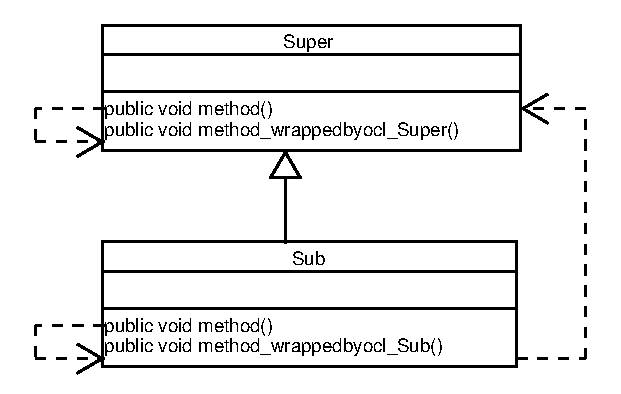
\includegraphics{WrapperLoop3.eps}} \par}
\vspace{0.3cm}

Wrapped methods get the class name appended. Thus, a wrapper method can call
the wrapped method of it's own class.


\subsection{Cleaning the Code\label{Sec:cleaningCode}}

Reversable modification means, that the injector is able clean the modified
code without leaving any traces. This section explains, how this requirement
is met. 

The user code is modified in two different ways only:

\begin{enumerate}
\item Renaming the wrapped methods/constructors.
\item Adding new object features, i.e. wrapper methods, methods for checking invariants
and observing attributes.
\end{enumerate}
For each method to be wrapped the suffix \texttt{\_wrappedbyocl} is appended
to the name. This transformation is done on the unparsed method header, so all
typographical extras (line breaks, comments etc.) are preserved. This transformation
is easily reversed, when the code has to be cleaned. For constructors, this
works similarly with appending the dummy parameter to the parameter list.

Removing generated class features relies on the fact, that the injector tags
all generated features as shown below.

\begin{lyxcode}
/{*}{*}\\
~~~@author~ocl\_injector\\
{*}/\\
void~checkOclInvariants();
\end{lyxcode}
When cleaning the code, the injector simply removes all object features carrying
such an \texttt{@author} tag. This is quite simple and functional.


\subsection{Design of the Java Parser\label{sec: JavaParser}}

Previous sections stated, that a very simple parser is sufficient for implementing
wrapper methods. This is proofed in this section by giving an overview of the
parsers design. In fact, it's as simple as a parser used for syntax highlighting
and class browsers in a java IDE.

First, the parser is actually a manipulator. The java file is simultaneous read,
parsed, modified on-the-fly and written to an output file. For a class diagram
of the parse tree produced see figure \ref{fig: JavaParser}.

\begin{figure}
{\centering \resizebox*{10cm}{!}{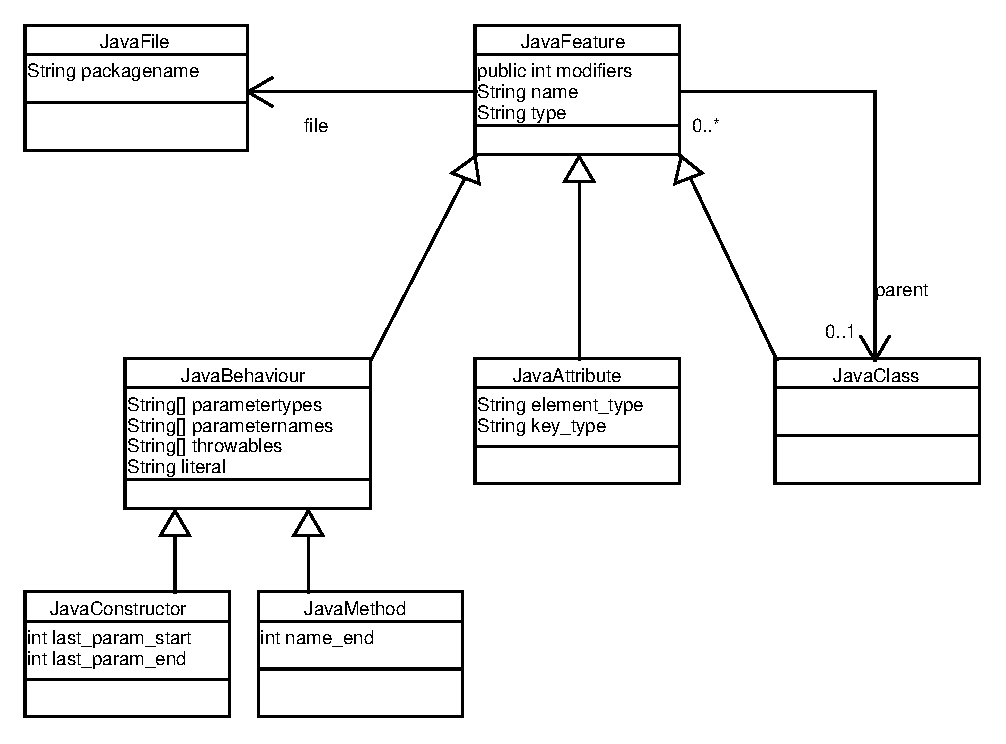
\includegraphics{JavaParser.eps}} \par}


\caption{Design of Java Parser \label{fig: JavaParser}}
\end{figure}

The parser analyses things which are relevant for the parse tree only. Particularly
method bodies and attribute initializers are ignored. These skipped parts may
not even compile. As long as the parenthesis balance is held, the java parser
will process them correctly.


\subsection{Comparison to Jass\label{sec: compareJass}}

Jass (\cite{jassWeb}) is a precompiler for checking assertions in java. It
translates jass files into java. Jass files are valid java source code with
assertions specified in comments. The generated java file contains additional
code checking these assertions. Thus, jass performs something similar to code
injection presented in the sections above. 

However, jass directly inserts generated code into user code as described in
section \ref{sec: SimpleApproach}. Thus the problems found there should occur
in jass too:

\begin{enumerate}
\item \emph{The code to be executed after the method has to be inserted before any
return statement.}\\
This is done by jass. Thus, it requires a full java parser (JavaCC here).
\item \emph{The return expression has to be computed in advance.}\\
This is also done by jass.
\item \emph{There may be name conflicts beetween the original and the generated code.}\\
Jass just defines a number of names (i.e. \texttt{jassResult}), which cannot
be used in the user code.
\item \emph{For methods with return type void it must be decided, whether the end
of the method is a reachable point of code.}\\
This is a known problem of jass. It will simply fail in such cases. There is
a work around: enclose the method body into a \texttt{if(true)\{...\}} statement.
\end{enumerate}
Jass performs a complex modification of the java source code. This modification
cannot be reversed as described in section \ref{Sec:injection_requirements_reversable}.
Thus, jass must be run before compilation whenever the source code has changed.
Additionally, the source code repository must hold jass files instead of java,
which causes lots of inconvenience for existing projects.

Jass cannot use wrapper methods, since this would not allow loop invariants
and check statements to be implemented. But without these features as in ocl,
method wrappers are much better than direct injection.


\section{Scope of Invariants\label{Sec:temporalScope}}

This section discusses the issue, when an constraint is required to be fulfilled.
This is trivially for pre/post conditions, but for invariants it's not so easy.

\cite{Warmer} section 5.4.2 suggests to check invariants immediately after
an object has changed\footnote{
This is partially corrected in the errata \cite{WarmerErrata}.
}. This is not workable, even if runtime efficiency is ignored. Modifications
on the model often produce intermediate states, which are not consistent according
to the constraints. 

When using databases the answer is simple: invariants must be valid outside
of transactions. Since the java system does not provide transactions, the code
injector offers several strategies for various user requirements.

Invariants may be required to be fulfilled on:

\begin{itemize}
\item All methods. This may be too strict, since private methods may intentionally
leave an object in an inconsistent state. 
\item Public methods (or any other access modifier). This may be not strict enough.
\item Tagged methods. A special tag in the documentation comment declares, that a
method promises to leave the system in a consistent state. This tag is then
part of the interface contract. This is the best solution, but requires additional
effort spent by the developer.
\item Explicit request. This is the way of choice, if the model is held in a database
backend. Then the checking of invariants is simply done immediately before committing.
\end{itemize}
These strategies may be used in conjunction. Except of \emph{All Methods} together
with \emph{Public Methods} and/or \emph{Tagged Methods} all other combinations
make sense for special user requirements.

There won't be a single solution for this problem. Many applications will require
their own individual scope of invariants. The scope may even differ beetween
several classes of invariants. 

Current implementation supports scopes needed during the ongoing diploma thesis
only. Up to now, all invariants share the same scope. Also, tagged methods are
not yet supported.


\section{Caching Results of Invariants\label{Sec:structuralScope}}

The previous section discussed, when we have to make sure, that all invariants
are fulfilled. But even then it's not absolutely necessary to evaluate all invariants.
The implementation developed along with this paper checks only those invariants,
whose result may possibly have changed by recent changes of the model.


\subsection{Design}

Caching is realized with an observer design. Each invariant determines all object
attributes it depends on and registers to these attributes as observer. Figure
\ref{Abb:observingInvariants} shows the meta model of the principal design.

\begin{figure}
{\centering \resizebox*{1\columnwidth}{!}{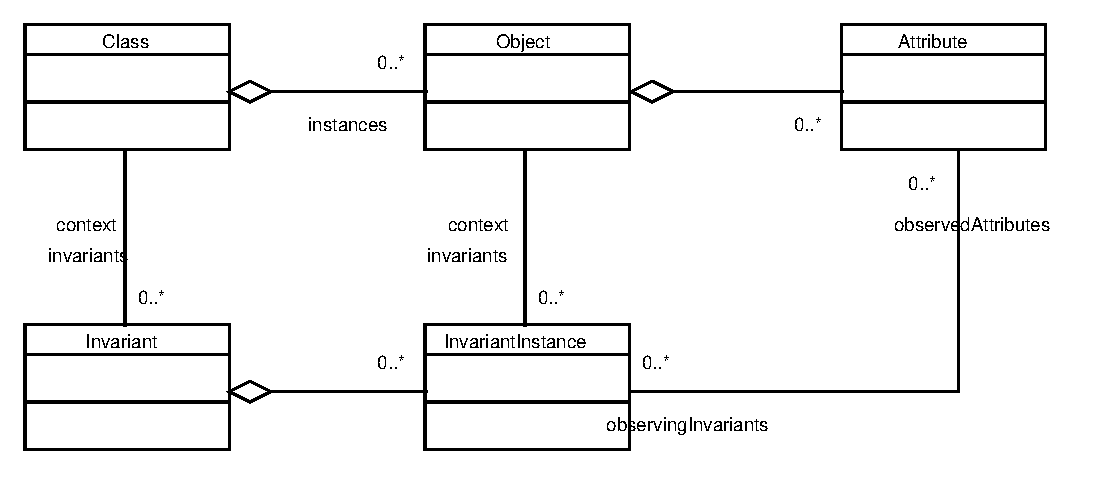
\includegraphics{observingInvariants.eps}} \par}


\caption{Design for Observing Invariants\label{Abb:observingInvariants}}
\end{figure} 

The classes in the UML chart have the following meaning:

\vspace{0.3cm}
{\centering \begin{tabular}{|l|p{5cm}|p{3cm}|}
\hline 
Class&
&
Example\\
\hline 
\hline 
Class&
An arbitrary class of the user model&
\texttt{class~Person}\\
\hline 
Invariant&
An invariant in the context of a class&
\texttt{context~Person~inv:~age>=0}\\
\hline 
Object&
An instance of a class&
Person John\\
\hline 
InvariantInstance&
An invariant in the context of an object.&
Has John a positive age?\\
\hline 
Feature&
A feature (attribute or query method) of an object.&
John's age\\
\hline 
\end{tabular}\par}
\vspace{0.3cm}

For now, lets think of features as attributes only. How to deal with query methods
is explained below. 

The cycle of checking invariants contains two stages.

\begin{enumerate}
\item Evaluating invariants. When evaluating an invariant instance, this invariant
instance registers to all object attributes used during evaluation as observer.
This means, the attribute promises to notify the invariant instance, when the
attributes value changes.
\item Running the model. When an attribute changed its value during execution of user
code, it notifies all observing invariant instances. Then, the attribute unregisters
all observers, so they must register again on the next evaluation stage.
\end{enumerate}
This design can be extended to query\footnote{
Operations used in ocl expressions must not have side effects.
} methods. If the query does not have parameters, it's exactly like attributes.
Things get a bit more complex, if the queries are parameterized. See figure
\ref{Abb:observingMethods}.

\begin{figure}
{\centering \resizebox*{1\columnwidth}{!}{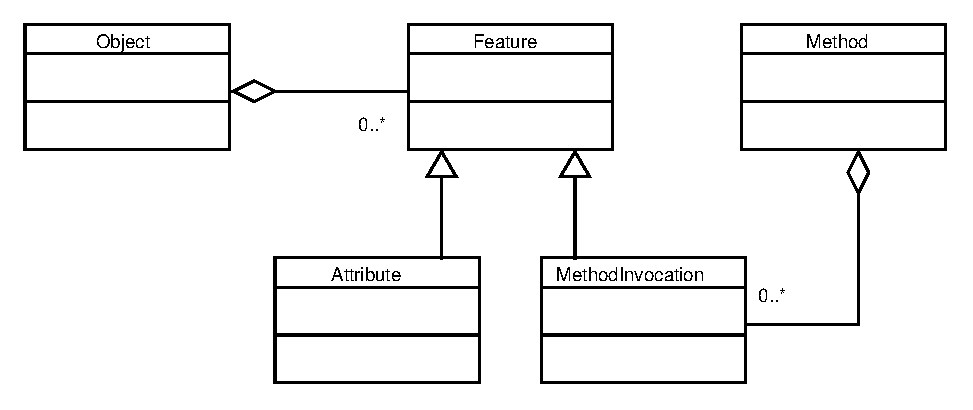
\includegraphics{observingMethods.eps}} \par}


\caption{Design for Observing Methods\label{Abb:observingMethods}}
\end{figure}

The point is, that not methods but method invocations are features observed
by invariants. A method invocation is a method together with a parameter sequence
suitable to invoke this method. 

Up to now, the implementation observes attributes only.


\subsection{Implementation}

Not all of these classes exist explicitly in the implementation. \emph{Class}
and \emph{Object} are provided by the user model already. \emph{Invariant} exists
only as an additional method \texttt{checkOclInvariant\_<name>} of its context
class. \emph{InvariantInstance} is an explicit class\footnote{
called a bit confusingly \texttt{tudresden.ocl.injection.lib.Invariant}.
} of the injection library. Finally \emph{Feature} is provided by the user model,
but cannot be referred as a single java object. (\texttt{java.lang.reflect.Field}
is a field of a class, not of an object.) Whenever a feature has to be referred,
it is represented by it's observer collection object, which sufficient for the
needs of this implementation.

Changes of object features are detected with polling. For each feature the ocl
injector adds a backup to the class. 

\begin{lyxcode}
class~Person\\
\{\\
~~int~age;\\
~~int~age\_oclbackup=age;\\
\}
\end{lyxcode}
Additionally there is a utility method added comparing each attribute to it's
backup. If there is a difference, the observers of the attribute are notified. 

\begin{lyxcode}
private~void~checkForChangedFeatures()\\
\{\\
~~if(age!=age\_oclbackup)\\
~~\{\\
~~~~age\_oclbackup=age;\\
~~~~//~notify~observers~of~age\\
~~\}\\
~~//~...~further~attributes\\
\}

~
\end{lyxcode}
This method is called immediately before and after each method of the class.
If the attribute contains an object reference, the comparison tests object identity,
not object equality. This means, the \texttt{!=} operator is used as for basic
types and not the \texttt{equals()} method. For collections the backup stores
a hashcode\footnote{
see \texttt{tudresden.ocl.injection.HashExact.identityHashCode}.
} of the collection to avoid the overhead of maintaining a complete backup collection.


\chapter{Model Information}

The OCL compiler needs model information for type checking. How this works is
explained in \cite{ff3} section 5.3.3. 

One possible source of model information may be a UML model exported from a
CASE tool. This is probably the most elegant way. But since most real-world
projects don't have a (up to date) UML representation of their business model,
this isn't feasible in practice.

Another source is the java code itself, accessed through reflection API\footnote{
see class \texttt{tudresden.ocl.check.types.ReflectionFacade}.
}. This very convenient, since no additional model is needed. However, java reflection
lacks some model properties which are important for type checking.

\begin{enumerate}
\item Element types of collections, particularly collections representing associations.
From a C++ perspective, java lacks templates implementing parameterized container
classes.
\item Qualifier types of maps, representing qualified associations.
\item The isQuery tag of operations. Note, that OCL expressions may use operations
without side effects (queries) only.
\end{enumerate}
This chapter present a solution to the first two items above. The information
needed is put into the source code. Section \ref{Sec:element_type_tag} explains,
how this information is stored, while section \ref{Sec:ReverseEngineering}
presents several approaches, how this information is generated.


\section{Representing Element Types\label{Sec:element_type_tag}}

Element types and qualifier types are specified special tags in java documentation
comments. See the example below. 

\begin{lyxcode}
class~Company\\
\{\\
~~/{*}{*}\\
~~~~~All~persons~employed~by~this~company.\\
~~~~~@element-type~Person\\
~~{*}/\\
~~Collection~employees;\\
\}
\end{lyxcode}
The \texttt{@element-type} tag has a syntax like \texttt{@see} as defined in
\cite{JAVA} section 18.4.1, but may refer to classes and interfaces only. This
tag is valid for attributes only, and there may be only one of such tags per
documentation comment. The tag is not restricted to attributes of type \texttt{java.util.Collection},
since future implementations could use other collection API's as well.

Analogously, the \texttt{@key-type} tag is introduced for association qualifiers. 

\begin{lyxcode}
class~Bank\\
\{\\
~~/{*}{*}\\
~~~~~Customers~qualified~by~their~account~number.\\
~~~~~@element-type~Person\\
~~~~~@key-type~Integer\\
~~{*}/\\
~~Map~customers;\\
\}
\end{lyxcode}
Note, that the reflection model is restricted to qualified associations with
one qualifier only. \cite{UML} allows multiple qualifiers, but there is no
convenient representation for this in java. 

Furthermore, UML specifies the unqualified association feature to be a set,
i.e. there must be no duplicates. Since this is not enforced by \texttt{java.util.Map}
(only keys are guaranteed to be unique), the ocl library provides an appropriate
runtime check.


\paragraph{Implementation.}

A really comfortable implementation would let the java compiler do the parsing,
and provide the information through an extended reflection API. This would be
similar to the \texttt{@deprecated} tag. My implementation extends\footnote{
Encapsulated in \texttt{tudresden.ocl.check.types.ReflectionExtender}.
} the reflection facade by scanning the source code for these comments on demand.
This implies, that the java source code is necessary for type checking OCL constraints
in addition to the class files.

There is a crucial question left: Where do the tags come? Possible sources are:

\begin{itemize}
\item A UML model. The code generator of a CASE tool could generate these tags. 
\item Maintained by hand. It is good-practice of programming, to specify which kind
of objects are supposed to be in a collection attribute. The tags just make
this information available formally. 
\item Reverse Engineering. This is discussed in detail in section \ref{Sec:ReverseEngineering}
below.
\end{itemize}
Collection attributes with type tags are verified on runtime by the injected
code. Note, that this kind of type information is useful for reverse engineering
a UML model from given java code.


\section{Reverse Engineering\label{Sec:ReverseEngineering}}

Section \ref{Sec:element_type_tag} explained, how to store additional type
information of a java model in java documentation tags. This section discusses,
how to create this information.

Actually, these type tags have to be created manually. This chapter tries to
support the developer with an interactive tool for injecting \texttt{@element-type}
and \texttt{@key-type} tags into the code. There are two main features of this
tool:

\begin{enumerate}
\item Graphical User Interface: Clear presentation of missing type tags and comfortable
editing facilities. 
\item Decision Support: Giving hints to the developer. These hints are either derived
statically (section \ref{Sec:ReverseEngineeringStatic} and \ref{sec: ReverseEngineeringWomble})
or gathered dynamically on runtime (section \ref{Sec:ReverseEngineeringDynamic}).
There is a special indication, if several hints suggest different types.
\end{enumerate}
A prototype of this tool has been developed by Steffen Zschaler\footnote{
run class \texttt{tudresden.ocl.injection.reverseeng.RevengGUI}.
}.


\subsection{Source Code Analysis\label{Sec:ReverseEngineeringStatic}}

Information about element types may be derived from static properties of the
class, such as parameter types of methods and other tags in doccomments. 

The following example suggests some of these properties. The element type of
\texttt{employees} is obviously \texttt{Person}, but this information is not
yet available to the OCL compiler. The tool can derive an appropriate hint for
the developer from one of the underlined features.

\begin{lyxcode}
/{*}{*}\\
~~~All~employed~\{@link~\underbar{Person}~persons\}~of~this~company.\\
~~~@see~\underbar{Person}\\
{*}/\\
Collection~employees;\\
~\\
boolean~isEmployee(\underbar{Person});\\
void~addEmployee(\underbar{Person});\\
void~removeEmployee(\underbar{Person});
\end{lyxcode}
Note, that the example above requires linguistic knowledge about plural and
singular form of nouns (employee here). This gets far more difficult, if identifiers
are not English.


\subsection{Runtime Analysis\label{Sec:ReverseEngineeringDynamic}}

This section describes, how to trace element types of collections on runtime.
This is useful, if there is no static type information available, as described
in the previous section. 

For each collection attribute, the object types encountered during a run of
the program are collected and fed into the interactive tool. This requires the
program to be executable. Additionally there must be extensive test cases available,
otherwise only a subset of all possible element types will be encountered.

The interactive tool presents the set of object types for every collection attribute.
Additionally, the tool highlights all types, for which there is no super type
in this set. Formally, this are the local minima of the set respective to the
generalization partial order. These local minima are good candidates for a element
type, especially if there is only one minimum. Presenting minima simplifies
the decision if there are many types encountered in the collection attribute.


\paragraph{Implementation.}

The ocl injector makes a static method \texttt{traceTypes}\footnote{
actually \texttt{tudresden.ocl.injection.lib.TypeTracer.traceTypes}.
} to be executed whenever a collection attribute changes it's contents. Class
\texttt{TypeTracer} maintains a static data structure containing all element
types and key types for all attributes, as well as the minima of these type
sets. This information is continuesly written to a log file. The interactive
tool reads this log file on startup.


\subsection{Byte Code Analysis \label{sec: ReverseEngineeringWomble}}

This section describes how type information can be extracted from java byte
code. This technology and it's implementation (called Superwomble) was developed
by Daniel Jackson and Allison Waingold at the MIT. This section outlines the
parts of their paper (\cite{womble}) related to type information together with
my experiences with the tool.

Superwomble is a powerful reverse engineering solution. It generates object
graphs from nothing but java byte code. Object graphs are roughly speaking a
subset of UML class diagrams. They feature classes with generalizationships
and associations beetween them. The graph is finally fed into a tool named dot,
which does a nice layout for the graph.

One of the tricky parts of this tool is the detection of element types for object
containers, which is exactly what this whole chapter is about. How this works,
is explained on the Company-Person example from section \ref{Sec:element_type_tag}
(page \pageref{Sec:element_type_tag}). 

Suppose \texttt{company} is a variable of type \texttt{Company} and \texttt{person}
of type \texttt{Person}. A typical program around this example would probably
contain a statement like this:

\begin{lyxcode}
company.employees.add(person);
\end{lyxcode}
The operation \texttt{add} takes an argument of type \texttt{Object}, but is
called with a variable of type \texttt{Person}. This is a good hint, that the
element type of employees is \texttt{Person}.

The same works for objects returned from the container. The expression

\begin{lyxcode}
person=(Person)(company.employees.iterator().next());
\end{lyxcode}
strongly suggests the element type \texttt{Person}.

Another highlight of superwomble is, that container classes are detected even
if they don't implement \texttt{java.util.Collection}. In fact the type is not
cared at all. Instead there are some heuristics applied to decide, whether a
class is an object container or not.

I used the tool on several parts of both the ocl toolkit and the net-linx code,
and it produced good and reliable results.

Integration of superwomble results into the interactive tool should be possible.
The object graph is exported to a human readable text file. However, this task
is outside the scope of this paper.


\subsection{Comparison}

This section provides a comparison beetween the three approaches presented in
the section above. 

\vspace{0.3cm}
{\centering \begin{tabular}{|l||c|c|c|}
\hline 
&
Source Code&
Byte Code&
Runtime\\
&
&
(Superwomble)&
\\
\hline 
\hline 
Source Code required&
yes&
no&
yes\\
\hline 
Required Code Quality&
fairly &
fully &
up and \\
&
parseable&
compileable&
running\\
\hline 
Availability of Results&
intermediate&
good &
good\\
\hline 
Reliability of Results&
good&
very good&
intermediate\\
\hline 
Application Effort&
low&
low&
high\\
\hline 
Implementation Effort &
low&
high&
very low\\
(starkly subjective)&
&
&
\\
\hline 
License&
LGPL&
Binary at no cost&
LGPL\\
\hline 
\end{tabular}\par}
\vspace{0.3cm}

Only byte code analysis requires no source code. This argument is weakened by
the fact, that the type information is to be inserted into source code anyway.
However, byte code analysis may cover libraries, which aren't available in source
code, but provide useful type information about other parts of the program.

Anyway, byte code analysis requires, that there is a fully compilable source
code somewhere, even if it's not available to the user. Source code analysis
even makes do with incorrect source code, as long as meta data is parsable (method
headers etc.) and method bodies hold the bracket balance. Most demanding on
source code quality is runtime analysis, which requires a running system, with
complete test cases.

Source code analysis is most demanding on the ``beauty'' of implementation.
To deliver results, it requires some kind of getter/setter methods for the container
attributes. In contrary, byte code and runtime analysis even work for public
container attributes manipulated from outside of the class.

For runtime analysis \emph{reliability of results} depends heavily on completeness
of test cases. If the test cases are insufficient, results may be wrong. Byte
code analysis provides best reliability, it's more difficult for a poor quality
code to fool the analysis.

Runtime analysis also requires most \emph{application effort} for the user.
The system must be actually run. Particularilly all requirements for runtime
(libraries, database, configuration etc.) must be available.

The \emph{implementation effort} is very subjective for this paper. Both source
code and runtime analysis require a java parser and injector, which was already
built for code injection. Thus the implementation effort for me was low. Byte
code analysis is something completely different.

Finally, \emph{license} is about whether it is allowed to use, review and adapt
the implementation. Roughly speaking, the difference beetween \emph{LGPL} and
\emph{Binary at no cost} is same as beetween free speech and free beer (\cite{freesw}).


\subsection{Summary}

There have been three approaches presented for acquiring type information. Source
code and runtime analysis are implemented and fully integrated into the project.
Experiences with byte code analysis where drawn from the tool superwomble (\cite{womble}).
This is fully implemented but not integrated into the ocl toolkit, thus not
ready to use.

Adding up the scores, byte code analysis is probably the best. However, most
of the criteria listed above are some kind of orthogonal, so adding up scores
might not be sufficient for a decision. Each application may emphasize different
criteria, so a universal solution is not available.

All approaches have one thing in common: they are not perfect. Thus, they cannot
be used directly in the type checker of the ocl compiler. The intermediate step
of the \texttt{@element-type} tags is necessary to allow correcting user intervention.


\chapter{Maintaining the OCL Compiler}

This chapter describes all major changes to Frank Fingers OCL compiler. This
includes bugfixes too, if they caused changes of internal or external interfaces.
It it some kind of update for \cite{ff3}, listing everything changed since.


\section{Reflection Facade and OCL Library}

Many changes occurred both in the reflection type facade and in the ocl library.
This section groups these changes.


\subsection{Polymorphism of Operation Parameters}

Both \texttt{ReflectionFacade.\-navigateParameterized} and \texttt{OclAnyImpl.\-getFeature}
lacked polymorphism of operation parameters. This means, that a method is found
only if actual parameter types match formal parameter types exactly. The correct
behavior is, that actual parameter types may also be subtypes of formal parameter
types. For a detailed description see \cite{rw7} section 3.1.5. 

The new implementation made \texttt{ReflectionAdapter.\-getClassForType} superfluous,
so it was removed from the interface.


\subsection{Mandatory Name Adapters}

Previous versions of the ocl library provided a default functionality, if no
name adapter had been set explicitly.

Now its mandatory to set a name adapter. Otherwise a NullPointerException is
thrown. The default functionality has been moved into a separate name adapter
(\texttt{SimpleNameAdapter}) which is used in the reflection facade as well.
The name adapter may also be set by the java property \texttt{tudresden.ocl.lib.nameadapter}.


\subsection{Qualified Associations}

The OCL support was enhanced by adding a simplified form of qualified associations
to the reflection facade and the ocl library. ``Simplified'' means, that there
may be only one qualifier attribute. 

Qualified associations are represented in java with \texttt{java.util.Map} by
default, but this may be changed by implementing \texttt{ReflectionAdapter.isMap()}.


\subsection{Type Mapping from OCL to Java.}

The mapping beetween ocl types and java types now supports the collections API
introduced in JDK version 1.2. The changes concern \texttt{DefaultOclFactory.\-getOcl\-Representation\-For(Object)}
and \texttt{DefaultReflection\-Adapter.getClass\-ForType}. 

A special handling of \texttt{java.util.Vector} supports code generated by Argo/UML.
The static configuration variable \texttt{Ocl.TAKE\_VECTORS\_AS\_SET} causes
vectors to be mapped to sets, instead of sequences.

The new mapping is listed below.

\vspace{0.3cm}
{\centering \begin{tabular}{|c|c|c|}
\hline 
Java (java.util)&
take vectors as set&
OCL\\
\hline 
\hline 
List&
-&
Sequence\\
\hline 
Vector&
false&
Sequence\\
&
true&
Set\\
\hline 
Set&
-&
Set\\
\hline 
Map&
-&
Set (qualified)\\
\hline 
\end{tabular}\par}
\vspace{0.3cm}

Furthermore, arrays are now supported. They are mapped into sequences of the
appropriate element type.


\section{Undefined Values in the OCL Library}

Previous versions of the ocl library implemented undefined values as singletons
for each type. 

This was given up. Now undefined values carry the reason for their creation
with them. When the undefined value is tried to be evaluated, this reason is
added to the exception message. 

This made \texttt{Ocl.STRICT\_CHECKING} superfluous, so it was removed. replaced
exceptions by undefined values, parameterized with the reason for the undefined
value.

Additionally some other parts 

\begin{enumerate}
\item Method \texttt{OclCollection.setToRange} now creates an undefined collection
(instead of throwing an exception), if lower bound is greater than upper bound.
\item The methods \texttt{Ocl.to<OclType>(OclRoot)} now return a undefined value of
the appropriate type, if argument is undefined. 
\end{enumerate}

\section{Typechecker}

\begin{enumerate}
\item added OclAny to TypeChecker (DefaultTypeFactory). 
\item Bugfix, removed TypeFactory.getClassifier - replaced all calls by TypeFactory.get
\end{enumerate}

\section{JavaCodeGenerator: \label{Sec:maintainJavaCodeGenerator}}

\begin{enumerate}
\item different meaning of Codefragments created for @pre expressions (TRANSFER, PREPARATION,
CODE), makes it easier and more flexible for different code injector tools.
compare to \cite{ff3} section 7.1.2, description of new behavior in section
\ref{Sec:codegeneration_result}, TODO comparison to Franks example
\item explicit package qualifier for ocl library is optionally prepended. Replaces
the import statement and therefore fulfills the corresponding requirement in
section \ref{Sec:injection_requirements}.
\end{enumerate}

\section{Silly Bugfixes}

\begin{enumerate}
\item JavaCodeGenerator: order on arrow
\item Basic.navigate: max{[}1{]}
\item DefaultOclFactory.getOclRepresentationFor(Object): dealing with Float and Double
\item OclCollection.setToRange: exchanged bounds in error condition
\end{enumerate}
\appendix

\chapter{Usage of Injector }

This chapter describes, how to use the injector tool. 

Synopsis is below.

\begin{lyxcode}
java~tudresden.ocl.injection.Main~{[}options{]}~file.java~...
\end{lyxcode}
Provide all java files, you want to modify. 

Options recognized are below. Most options have a short and a long version.
Long versions try to be self explanatory and should be used in scripts.

\begin{lyxcode}
-m~-{}-modify
\end{lyxcode}
\begin{quotation}
Enables modifying java files. If not provided, the modified java code is written
to \texttt{file.java.injected}. This switch serves as a safety check, whether
you \emph{really} want to replace your source code with the output of the injector.
\end{quotation}
\begin{lyxcode}
-c~-{}-clean
\end{lyxcode}
\begin{quotation}
Performs cleaning of source files instead of injection. After cleaning, the
source code should show no differences to the version before injecting.
\end{quotation}
\begin{lyxcode}
-f~-{}-constraint-file~constraints.txt
\end{lyxcode}
\begin{quotation}
Specifies the text file containing the constraints. Usually not needed, since
constraints may and should be placed into java doc comments. See section \ref{Sec:embedConstraints}.
\end{quotation}
\begin{lyxcode}
-x~-{}-xmi-model~model.xmi
\end{lyxcode}
\begin{quotation}
Specifies the XMI file containing the model covered. Is used for type checking
only. Use this only, if you cannot use \texttt{-{}-reflection-model}.
\end{quotation}
\begin{lyxcode}
-r~-{}-reflection-model~modelpackage
\end{lyxcode}
\begin{quotation}
Specifies the java packages containing the model covered. If there is a constraint
\texttt{context~Person}, the type checker will look for class Person in all
package given by this option. This is some kind of ``\texttt{import} for ocl''.
For multiple packages use multiple options.
\end{quotation}
\begin{lyxcode}
-n~-{}-name-adapter~{[}none|argo{]}
\end{lyxcode}
\begin{quotation}
Specifies the name adapter. Default is \texttt{none}. If you don't use code
generated by Argo/UML, the default is sufficient. Further information on name
adapters is available at \cite{ff3} section 3.5.1 and 3.5.6.
\end{quotation}
\begin{lyxcode}
-is~-{}-invariant-scope~{[}all|private|protected|package|public|explicit{]}
\end{lyxcode}
\begin{quotation}
Specifies the the scope of invariants used. See section \ref{Sec:temporalScope}
for a detailed explanation. Access modifiers select methods having the same
or a more public access modifier. Thus, \texttt{all} and \texttt{private} are
equivalent. Default is \texttt{all}.
\end{quotation}
\begin{lyxcode}
-vm~-{}-violation-macro~macro
\end{lyxcode}
\begin{quotation}
Specifies what to do, if a constraint fails. This string is inserted verbatim
into the code. The injector appends a pair of parents enclosing a suitable message
string. Good candidates are \texttt{System.out.println} (the default) or \texttt{throw
new~RuntimeException}. Note, that the latter must be enclosed in \texttt{\char`\"{}\char`\"{}}
on Unix shells.

The exception thrown must not be a \emph{checked exception} as specified by
\cite{JAVA} section 11.2. Otherwise the modified code will not compile!
\end{quotation}
\begin{lyxcode}
-tt~-{}-trace-types
\end{lyxcode}
\begin{quotation}
Performs type tracing of collection elements. See section \ref{Sec:ReverseEngineeringDynamic}
for details. The information gathered is written to a log file specified by
property \texttt{tudresden.\-ocl.injection.\-lib.TypeTracer.log}.

Note, that the log file must be specified when running the user program, not
the injector! For example use \texttt{-Dtudresden.\-ocl.injection.\-lib.TypeTracer.\-log=ocltypetrace.txt}.
If not specified, the type information is written to standard out.
\end{quotation}
\begin{lyxcode}
-{}-insert-immediately
\end{lyxcode}
\begin{quotation}
Triggers immediate insertion of wrapper methods. Otherwise wrapper methods are
inserted at the end of each class. Immediate insertion allows easier tracing
of the modifications. This option is mainly useful for debugging.
\end{quotation}
\begin{lyxcode}
-{}-trace-checking
\end{lyxcode}
\begin{quotation}
Adds code logging each constraint checked on an object to standard out. Useful
for debugging.
\end{quotation}
\begin{lyxcode}
-{}-simple-hash
\end{lyxcode}
\begin{quotation}
Uses simple hash functions in \texttt{HashSimple}, instead of the sophisticated
hash functions in \texttt{HashExact}. Simple hash functions just return the
size of the collection, so they will detect insertions/deletion only. Reduces
CPU load for big models.
\end{quotation}
\listoffigures

\begin{thebibliography}{WK99e}
\bibitem[FF00]{ff3}Frank Finger. Design and Implementation of a Modular OCL Compiler. Diplomarbeit.
TU-Dresden 2000. http://dresden-ocl.sourceforge.net/
\bibitem[WK99]{Warmer}Jos Warmer, Anneke Kleppe. The Object Constraint Language: Precise Modeling
with UML. Addison-Wesley, 1999.
\bibitem[WK99e]{WarmerErrata}Errata for \cite{Warmer}: http://www.klasse.nl/ocl-boek/errata.htm
\bibitem[UML]{UML}OMG Unified Modeling Language Specification, Version 1.3, June 1999.
\bibitem[OCL]{OCL}Object Constraint Language Specification. Chapter 7 in \cite{UML}.
\bibitem[JAVA]{JAVA}James Gosling, Bill Joy, Guy Steele. The Java Language Specification. Edition
1.0. August 1996.
\bibitem[JW99]{womble}Daniel Jackson, Allison Waingold. Lightweight Extraction of Object Models from
Bytecode. Proc. International Conference on Software Engineering. May 1999.
http://sdg.lcs.mit.edu/womble/
\bibitem[KSR00]{kbeans}Holger Knublauch, Martin Sedlmayr, Thomas Rose. Design Patterns for the Implementation
of Constraints on JavaBeans. http://www.faw.uni-ulm.de/kbeans/
\bibitem[DB99]{jassDiplom}Detlef Bertetzko. Parallelit�t und Vererbung beim \char`\"{}Programmieren mit
Vertrag\char`\"{} - Weiterentwicklung von JaWA (in german). Master Thesis. Universit�t
Oldenburg 1999.
\bibitem[JASS]{jassWeb}The Jass Page. http://semantik.informatik.uni-oldenburg.de/\~{}jass/.
\bibitem[MMS]{JMSAssert}Man Machine Systems. JMSAssert. http://www.\-mmsindia.\-com/\-JMSAssert.html.
\bibitem[iCt]{iContract}iContract. http://www.reliable-systems.com/tools/iContract/\-iContract.htm.
\bibitem[ELX]{elixir}Elixir Technology Pte Ltd. http://www.elixirtech.com/index.html
\bibitem[CMA]{CodeInstrumentation}Glen McCluskey \& Associates LLC. Java Test Coverage and Instrumentation Toolkits.
http://www.\-glenmccl.\-com/\-instr/\-index.htm
\bibitem[CIG]{Cybernetic}Cybernetic Intelligence GmbH. OCL Compiler. http://www.\-cybernetic.\-org/\-prodocl.htm
\bibitem[OIJV]{jvision}Object Insight, Inc. JVISION. http://www.\-object-insight.\-com/\-html/\-product\_info.html
\bibitem[RW00]{rw7}Ralf Wiebicke. XML Query Languages for Repositories Based on XML Documents.
Gro�er Beleg. TU-Dresden 2000. http://dresden-ocl.sourceforge.net/
\bibitem[FSF00]{freesw}Free Software Foundation. What is Free Software? 1996-2000. http://www.gnu.org/philosophy/free-sw.html
\end{thebibliography}
\end{document}
